
\parindent0pt

\begin{minipage}{1.05\textwidth}
\vspace{\baselineskip}
\parindent0pt
\fboxrule0pt
{
\centering
\fbox{\centering
\begin{minipage}[t]{0.89\textwidth}
\centering
\begin{minipage}[t]{0.41\textwidth}
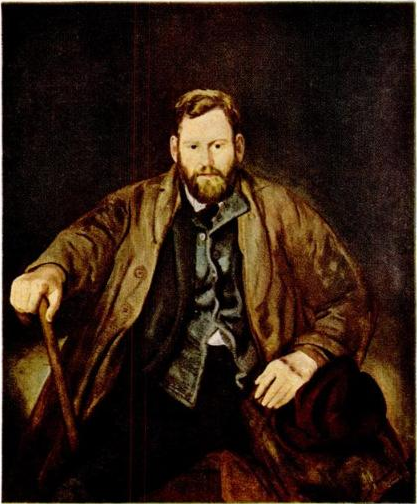
\includegraphics[width=1\textwidth]{./images/threewomen01.png}\vspace*{-8pt}%
\captionof*{figure}{\noindent\footnotesize\textbf{WALDO PEIRCE}, a famous painting in his own right,
turned model for Bellows, posed for this impressive portrait in New York studio in 1920.}
\end{minipage}\hspace{0.5cm}
\begin{minipage}[t]{0.4\textwidth}
   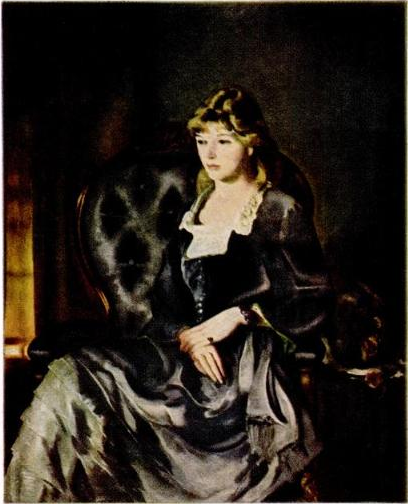
\includegraphics[width=1\textwidth]{./images/threewomen02.png}\vspace*{-8pt}
    \captionof*{figure}{\noindent\footnotesize\textbf{MRS KATHERINE ROSEN,}
                 the daughter of Charles Rosen, he was an artist and neighbor of bellows, 
                 posed for this  meditative study in 1921.}
\end{minipage}
\end{minipage}
}}

\medskip

\fbox{\hskip-0.3cm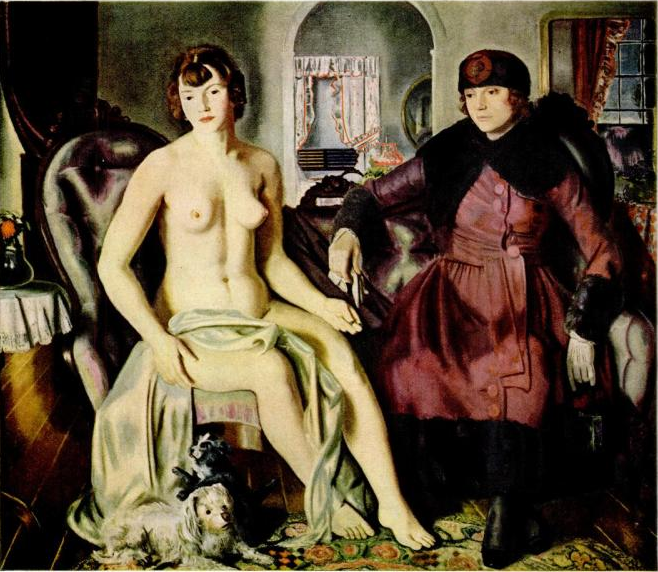
\includegraphics[width=1.03\textwidth]{./images/twowomen-03.png}}\\[-27.5pt]
\setlength{\linewidth}{.95\textwidth}
\setlength{\columnsep}{8pt}
\begin{multicols}{2}
\noindent \footnotesize\textbf{TWO WOMEN,} portrays a professional model dressed and undressed. The range and richness of colors is unusual among Bellows' pictures. Bellows always had a horror of studio pictures and ``pretty nudes,'' rarely worked from professional models and never painted a still life.
\end{multicols}
\vfill

\captionof{figure}{Balancing three images on a page. Should the larger image be at the top or at the bottom?}
\end{minipage}

\newcommand\articleheading[1]{%
    \par
    \vspace*{2\baselineskip}
    \bgroup
    \LARGE\bf\textsf{\noindent #1}
    \egroup
   \vskip2\baselineskip
}
\clearpage

\begin{minipage}{\textwidth}
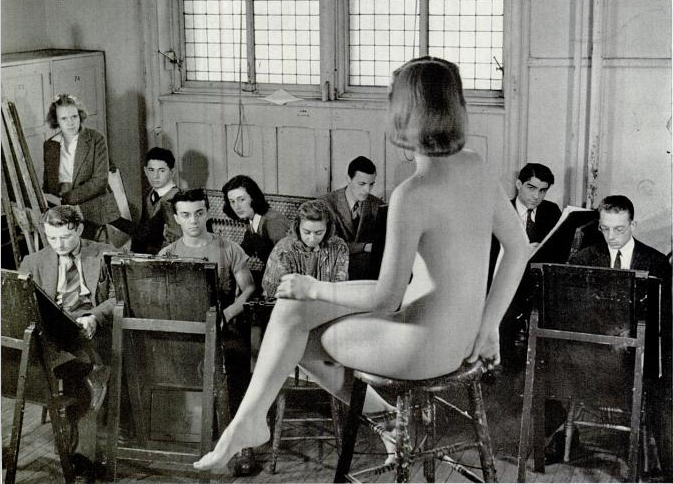
\includegraphics[width=\textwidth]{./images/yaleartschool.png}

\articleheading{TRADITION AND TECHNIQUE AT YALE'S SCHOOL OF  FINE ARTS}

\end{minipage}
\begin{multicols}{3}
        \lettrine{A}{t Yale}\lorem \lipsum[1-3]
        \par
\end{multicols}

\newgeometry{top=0pt, left=0pt, right=0pt, top=0pt, bottom=2cm}
\pagebreak

\begin{minipage}{\textwidth}
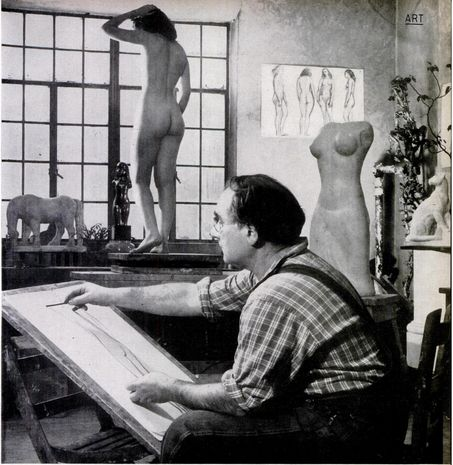
\includegraphics[width=\textwidth]{./images/sculpture-lesson.jpg}\par
\vspace{\baselineskip}

\centerline{\HUGE\bfseries SCULPTURE LESSON}
\vspace{0.5\baselineskip}

\centerline{\LARGE\bfseries Noted arist shows how adventurous amateurs can model with clay }

\end{minipage}

{
\leftskip1cm\rightskip1cm\columnsep-1.3cm\par\leavevmode

\begin{multicols}{3}
        \lettrine{A}{t Yale} \lorem \lorem \lorem \lorem
        
\end{multicols}
}

\newgeometry{top=1.5cm,left=2cm,right=2cm,bottom=2cm}

\pagebreak





\lipsum[1]
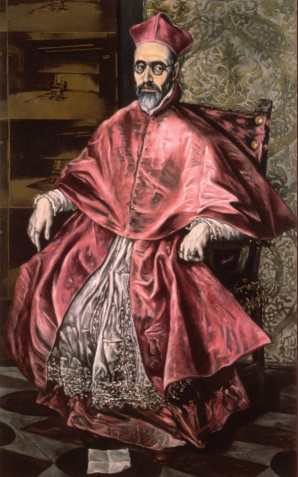
\includegraphics[height=0.8\textheight, width=\textwidth\relax]{./images/nino.png}

This is a short caption test and this one is a long caption test.

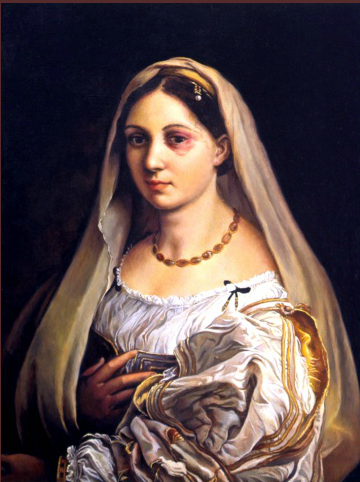
\includegraphics[width=\textheight, width=\textwidth]{./images/woman.png}
Donna Velata.

\clearpage
\raggedbottom


\noindent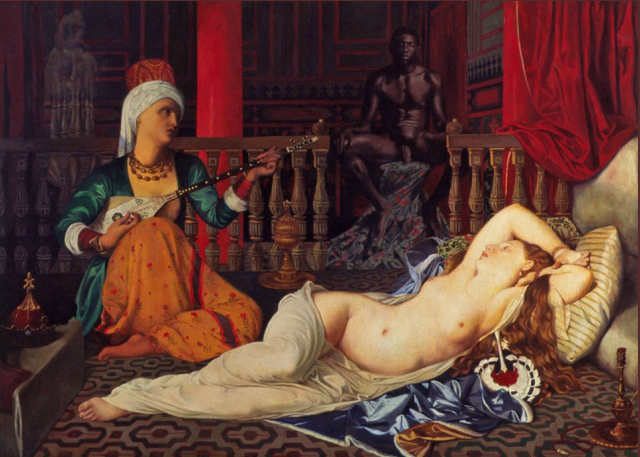
\includegraphics[width=\textwidth]{./images/odalisque.png}^^A
This is a short caption test and this one is a long caption test.
\vspace*{2\baselineskip}


\begin{minipage}[t]{0.3\textwidth}
\vbox to -6cm{\noindent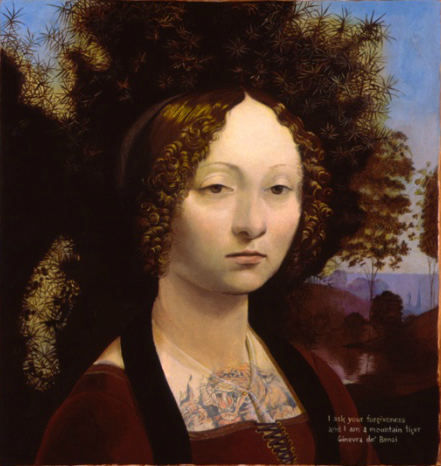
\includegraphics[width=0.98\textwidth]{./images/ginerva.png}
This is a short caption test and this one is a long caption test.}
\end{minipage}%
\begin{minipage}[t]{.7\textwidth}%
\noindent\textbf{\Huge \hfill Kathleen Gilje\hskip0.1em\hfill}\\[2\baselineskip]
\end{minipage}


\leftskip0.41\textwidth

Lorem ipsum dolor sit amet, consectetur adipiscing elit. Etiam eu nunc dolor. Nam arcu nisi, hendrerit at facilisis et, aliquet sit amet massa. Aenean ullamcorper mi dolor. Sed ut urna vitae elit tristique varius tempus vitae orci. Maecenas tristique lectus vel enim posuere congue. Aliquam pellentesque nisl vel nunc iaculis dictum. Sed luctus, orci vehicula blandit rutrum, risus justo aliquet elit, id venenatis est libero nec sem. Sed varius molestie ante non fringilla.

Vestibulum ut mollis odio. Vivamus ut risus eu dolor laoreet viverra. Nullam elit erat, congue at placerat ut, posuere non diam. Suspendisse eget dui et mi varius bibendum at non orci. Morbi justo arcu, posuere non tempus at, vestibulum sit amet lorem. Class aptent taciti sociosqu ad litora torquent per conubia nostra, per inceptos himenaeos. Donec tempor dignissim tellus, vitae vestibulum tellus hendrerit tempus. Nullam varius justo sit amet risus semper non semper eros placerat. Integer eleifend ligula in est gravida ornare tincidunt velit tristique.


Donec vel erat a ipsum condimentum volutpat vel non odio. Vivamus non justo orci. Pellentesque ligula ipsum, vestibulum at molestie vel, mollis sed odio. Donec rhoncus, sem in auctor tincidunt, libero quam scelerisque urna, et volutpat purus magna ac nulla. Cras vel quam nec urna viverra ornare eu et nibh. Pellentesque tincidunt leo non odio varius vitae sollicitudin neque adipiscing. 

\section{Full Page Images}

\leftskip0pt\parindent1em

In euismod, enim a dictum pharetra, libero nibh tempor enim, vel fermentum justo justo eget sem. Integer convallis massa nec turpis volutpat tristique. Quisque fringilla volutpat sem porta elementum. Donec vel metus quis nisl venenatis vehicula ac quis est. Maecenas vulputate lacinia lacus quis porttitor. Aliquam consectetur consectetur metus eu bibendum. Lorem ipsum dolor sit amet, consectetur adipiscing elit. In sem mauris, mollis nec pulvinar posuere, facilisis quis turpis. Quisque vel laoreet mauris.

Quisque ultrices dignissim odio at malesuada. Duis euismod tellus nec ante porta vel ullamcorper orci semper. Vivamus in eros est. Etiam et pellentesque nisi. Sed faucibus dictum tortor vitae accumsan. Donec ante risus, ornare et iaculis eget, cursus at metus. Maecenas neque urna, rutrum sit amet lacinia non, accumsan nec tortor. Proin tempor dictum porta. Morbi luctus nulla et sapien elementum aliquam ut eget neque. Quisque lobortis eleifend lorem adipiscing semper. Quisque molestie magna lorem, non mollis est. Mauris urna arcu, pretium sed dignissim id, tempor accumsan massa



\noindent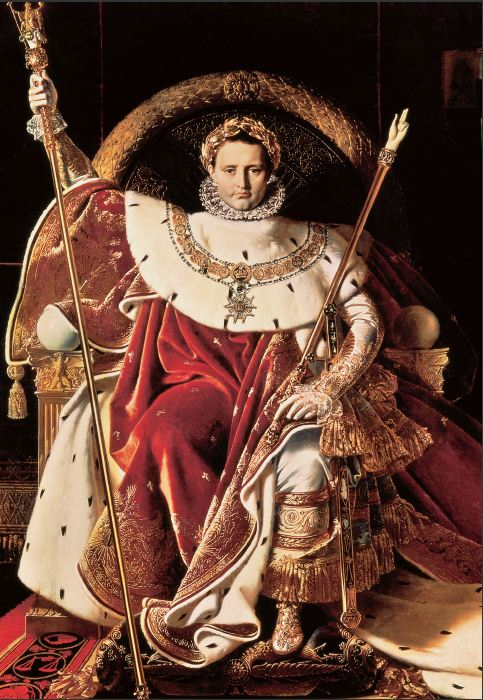
\includegraphics[width=\textwidth]{./images/napoleon.jpg}
This is a short caption test and this one is a long caption test.



\clearpage
\newenvironment{kathleen}[1][b]{\def\placement{#1}\parindent0pt
}{}

\cxset{kathleen align/.is choice,
       kathleen align/top/.code=\xdef\kathleenplacement@cx{t},
       kathleen align/bottom/.code=\xdef\kathleenplacement@cx{b},
       kathleen align/center/.code=\xdef\kathleenplacement@cx{c},
       kathleen imagei/.code=\def\imagei{\includegraphics[width=\textwidth]{#1}\par},
 kathleen imageii/.code=\def\imageii{\includegraphics[width=\textwidth]{#1}\par},
kathleen imageiii/.code=\def\imageiii{\includegraphics[width=\textwidth]{#1}\par},
kathleen imageiv/.code=\def\imageiv{\includegraphics[width=\textwidth]{#1}\par},
kathleen imagev/.code=\def\imagev{\includegraphics[width=\textwidth]{#1}\par},
kathleen captioni/.code=\def\captioni{\captionof{figure}{#1}},
kathleen captionii/.code=\def\captionii{\captionof{figure}{#1}},
kathleen captioniii/.code=\def\captioniii{\captionof{figure}{#1}},
kathleen scale/.store in=\kathleenscale@cx
}

\long\def\printkathleen{\begin{kathleen}[t]
\begin{minipage}{\kathleenscale@cx\textwidth}
\begin{minipage}[\kathleenplacement@cx]{0.3\textwidth}
\vbox{}
\imagei
\captioni
\imageii
\captionii
\imageiii
\captioniii
\end{minipage}\hspace{1cm}
\begin{minipage}[\kathleenplacement@cx]{0.46\textwidth}
\vbox{}
\imageiv
\captionof{figure}{This is a short caption test and this one is a long caption test.}\par
\imagev
\captionof{figure}{This is a short caption test and this one is a long caption test.}
\end{minipage}
\end{minipage}
\end{kathleen}}

\begin{figure}
\cxset{kathleen align = top,
       kathleen imagei = {./images/ladyagnew.png},
       kathleen imageii = {./images/etta.png},
       kathleen imageiii = {./images/etta.png},
       kathleen imageiv = {./images/ladyagnew.png},
       kathleen imagev  = {./images/etta.png},
       kathleen captioni = {Al contrario di quanto si pensi, Lorem Ipsum non \`e semplicemente una sequenza casuale di caratteri. Risale ad un classico della letteratura latina del 45 AC.}, 
       kathleen captionii = {Finibus Bonorum et Malorum di Cicerone. Questo testo un trattato su teorie di etica, molto popolare nel Rinascimento. La prima riga del Lorem Ipsum.},
       kathleen captioniii= This is a short caption.,
       kathleen scale = 1.1,
} 

\printkathleen

\caption{The Kathleen template page. It consists of five images and their caption text. Parameters can be set via a key value interface.}
\end{figure}
\clearpage

\cxset{kathleen align = top,
       kathleen imagei = {./images/ladyagnew.png},
       kathleen imageii = {./images/etta.png},
       kathleen imageiii = {./images/etta.png},
       kathleen imageiv = {./images/ladyagnew.png},
       kathleen imagev  = {./images/etta.png},
       kathleen captioni = {Al contrario di quanto si pensi, Lorem Ipsum non \`e semplicemente.}, 
       kathleen captionii = {Finibus Bonorum et Malorum di Cicerone. Questo testo  un trattato.},
       kathleen captioniii= This is a short caption.,
       kathleen scale = 0.7
} 

\cxset{kathleen align=bottom}




\begin{center}\printkathleen\par\label{kathleen}\end{center}

\newpage

\section{The Kathleen template} 

A lot of pages in image rich books have complicated settings for images.
These are difficult to manipulate and we provide here what we hope is
a better method. For example the Figure~\ref{kathleen} shows such a complex layout. This can be achieved by only filling in the template
values as shown below.

\begin{tcolorbox}
\begin{lstlisting}
\cxset{kathleen align = top,
       kathleen imagei = ladyagnew,
       kathleen imageii = etta,
       kathleen imageiii = etta,
       kathleen imageiv = ladyagnew,
       kathleen imagev  = etta,
       kathleen captioni = {Al contrario di quanto si pensi, Lorem Ipsum non \`e semplicemente una sequenza casuale di caratteri. Risale ad un classico della letteratura latina del 45 AC.}, 
       kathleen captionii = {Finibus Bonorum et Malorum di Cicerone. Questo testo un trattato su teorie di etica, molto popolare nel Rinascimento. La prima riga del Lorem Ipsum.},
       kathleen captioniii= This is a short caption.,} 
\cxset{kathleen align=bottom,
       kathleen scale=.5}

\printkathleen

\end{lstlisting}
\end{tcolorbox}


\newgeometry{top=0pt,left=1cm,right=1cm,marginparsep=0pt}

\clearpage


\parindent0pt
\pagestyle{empty}

\fboxsep0pt
\fboxrule0pt

\vspace*{-1cm}
\begin{minipage}{1.05\textwidth}
\hskip-0.9cm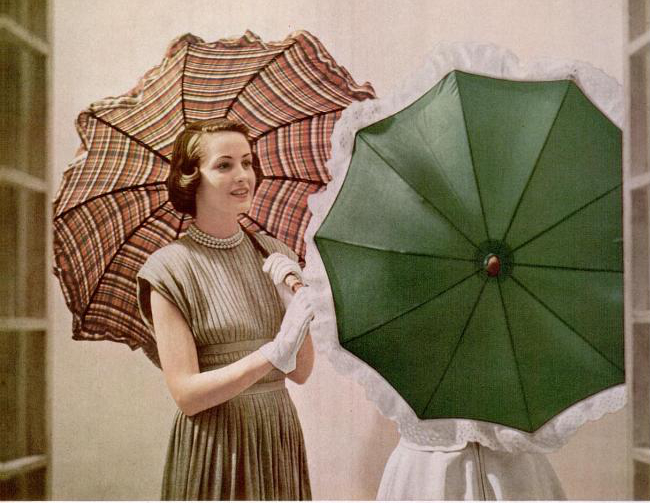
\includegraphics[width=1.03\textwidth]{./images/parasol-05.jpg}\\[-27.5pt]
\setlength{\linewidth}{0.95\textwidth}
\setlength{\columnsep}{10pt}
\begin{multicols}{2}
\noindent \footnotesize\textbf{DESIGNED FOR CONTRAST} with the wearer's ensemble, these plaid  tafetta and green rayon parasols, are best sellers at Maey's in New York. Set of matching parasol and shoes, or
gloves, scarves or bags, are also available to give simple dresses
a custom appearance.
\end{multicols}
\vspace{-0.25cm}
\rule{1.5cm}{0pt}\fbox{
\begin{minipage}[t]{0.87\textwidth}
\begin{minipage}[t]{0.41\textwidth}
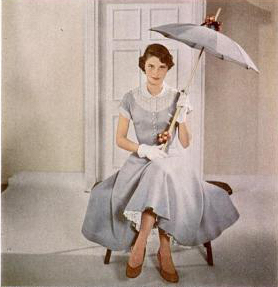
\includegraphics[width=1.03\textwidth]{./images/parasol-06.jpg}\par%
\noindent \footnotesize\textbf{CHERRY ORNAMENTS} adorn handle and tip of this parasol, made by Jane Derby to go with the afternoon dress. Straight handles are very popular.
\end{minipage}\hspace{0.5cm}
\begin{minipage}[t]{0.4\textwidth}
   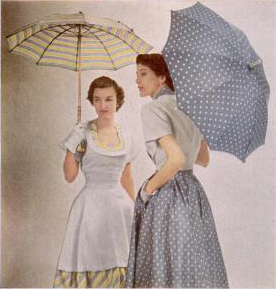
\includegraphics[width=1\textwidth]{./images/parasol-07.jpg}\par
\noindent \footnotesize\textbf{MATCHING SETS} of afternoon dress
and parasol, and four-piece polka dot weekend dress and parasol,
both designed by Briganne.
\end{minipage}
\end{minipage}
}

\vfill

\captionof{figure}{Balancing three images on a page. Should the larger image be at the top or at the bottom?}
\end{minipage}




\begin{minipage}{\textwidth}
\begin{minipage}[b][\textheight][b]{.47\linewidth}
\vspace*{2cm}

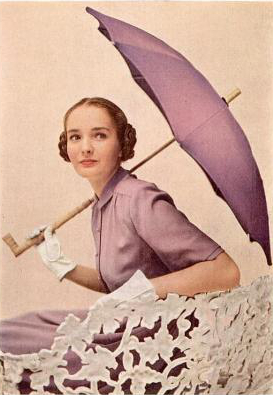
\includegraphics[width=\linewidth]{./images/parasol-03.jpg}\par
\vspace{2\baselineskip}

\centerline{\bfseries\Huge Parasols}
\vspace{2\baselineskip}

\begin{quote}
\lipsum[2]
\end{quote}

\vfill

\textbf{SHOES AND PARASOL SET} in pink are here combined with a dress, one of whose skirts is pink. Parasol is from New York's ``Uncle Sam'' parasol shop.
\end{minipage}\hspace*{1cm}
\begin{minipage}[b]{.53\linewidth}
\mbox{}
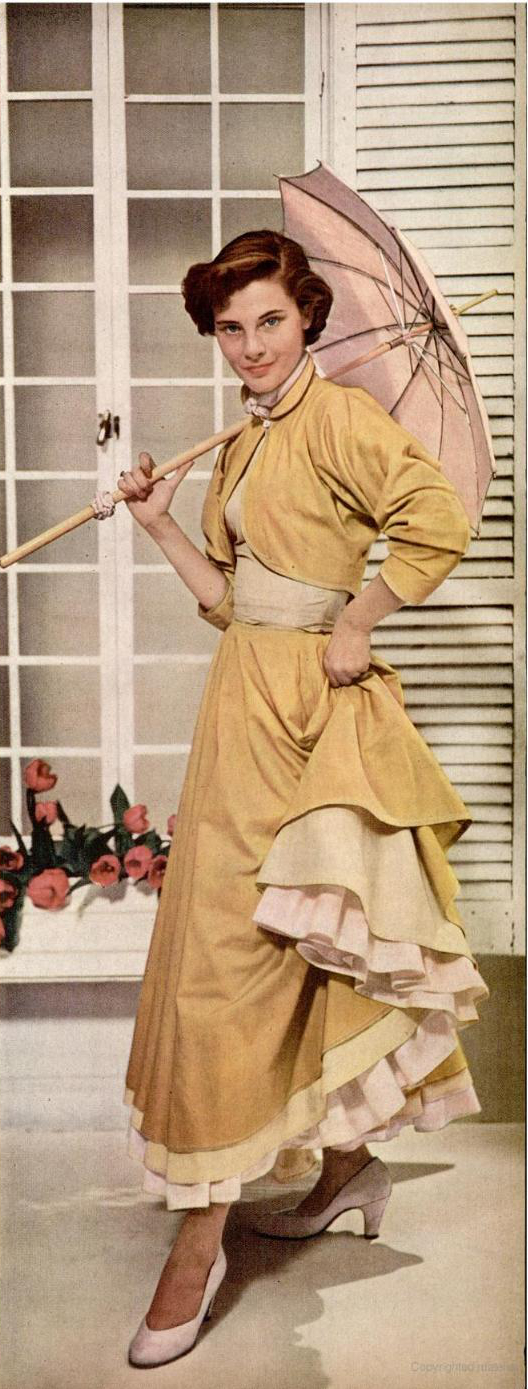
\includegraphics[width=\linewidth]{./images/parasol-01.jpg}\par
\end{minipage}
\end{minipage}

\newgeometry{top=1.5cm,bottom=3cm,left=3.5cm,right=3.5cm}

\clearpage